As was mentioned in Section~\ref{planByYears}, most of the first specific objective has been successfully developed. Its results derived in collaboration with experts from international institutions and two publications:

\begin{enumerate}
	\item Sanabria-Russo, L., Barcelo, J., Bellalta, B: ``Fairness in Collision-Free WLANs''. INFOCOM 2013 Student Poster Session, Turin - Italy. ArXiv e-prints (February 2013).\label{posterInfocom}
	\item Sanabria-Russo, L., Faridi, A., Bellalta, B., Barcelo, J., Oliver, M.: ``Future Evolution of CSMA Protocols for the IEEE 802.11 Standard''. Second IEEE ICC Workshop on Telecommunications Standards: From Research to Standards (June 2013).\label{ICCPaper}
\end{enumerate}

Results of publication~\ref{posterInfocom}~\cite{fairness-ECA} are summarized in Figure~\ref{fig:INFOCOMPoster}. The work includes the introduction of the concept of hysteresis and fair share to CSMA/ECA. It involved a thorough study of CSMA/ECA for then being able to adapt it to a simulation environment. 

For delivering the results, a modified version of the COST simulator~\cite{COST} was used. This tool separates the different components of the wireless networking communication (hosts, channel, queue and other components), permitting to modify their behavior independently.

Results from publication~\ref{ICCPaper}~\cite{research2standards} are contained in Figure~\ref{fig:ICCPaper}. Apart from showing the throughput enhancements over CSMA/CA, it is also shown how the proportion of collision slots reduces to zero in time when using CSMA/ECA. Furthermore, code snippets are presented to highlight the slight variations between CSMA/ECA and CSMA/CA.

\begin{figure}[htbp]
\centering
\begin{subfigure}{.5\textwidth}
  \centering
  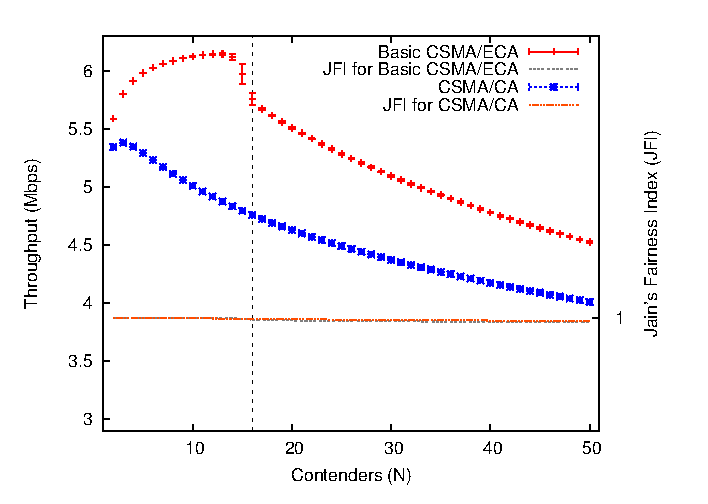
\includegraphics[width=\linewidth]{ECA-vs-CA-FINAL.eps}
  \caption{(a)}
  \label{fig:DCFvsECA}
\end{subfigure}%
\begin{subfigure}{.5\textwidth}
  \centering
  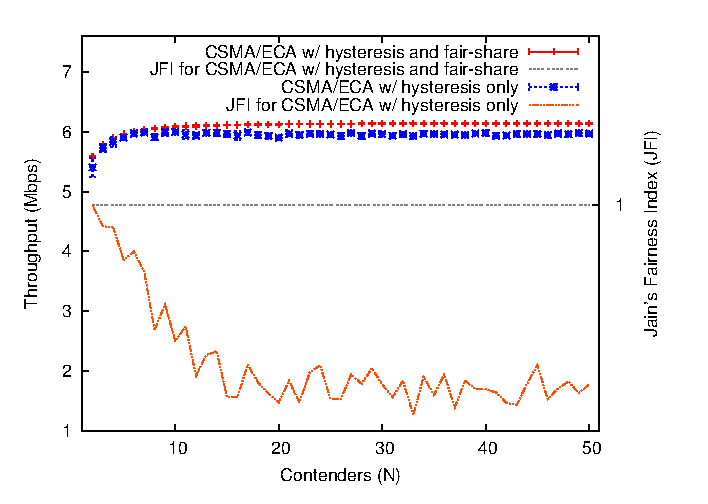
\includegraphics[width=\linewidth]{ECA-w-enhancements-FINAL.eps}
  \caption{(b)}
  \label{fig:ECAPerformace}
\end{subfigure}
\caption{\ref{fig:DCFvsECA}) Throughput of CSMA/CA vs. CSMA/ECA without hysteresis and fair share (referred to as Basic CSMA/ECA). \ref{fig:ECAPerformace}) Throughput and fairness when incorporating hysteresis and fair share to CSMA/ECA.}
\label{fig:INFOCOMPoster}
\end{figure}

\begin{figure}[htbp]
\centering
\begin{subfigure}{.5\textwidth}
  \centering
  \includegraphics[width=0.7\linewidth,angle=-90]{avgCollisions-12sta.eps}
  \caption{(a)}
  \label{fig:avgCollisions}
\end{subfigure}%
\begin{subfigure}{.5\textwidth}
  \centering
  \includegraphics[width=0.7\linewidth,angle=-90]{throughput-combined.eps}
  \caption{(b)}
  \label{fig:throughputCombined}
\end{subfigure}
\caption{\ref{fig:avgCollisions}) Cumulative fraction of slots spent in collisions for $N=12$ nodes. \ref{fig:throughputCombined}) Throughput.}
\label{fig:ICCPaper}
\end{figure}

Up until the date of this writing, only~\cite{fairness-ECA} has been presented. It took place at the $32^{nd}$ IEEE INFOCOM, April 14-19 at Turin, Italy. The conference provided the opportunity to meet with people involved in the FLAVIA and Wireless MAC Processors projects~\cite{FLAVIA,WMP}, which have been providing helpful assistance ever since. 

Between Jun 9-13 2013, the second work derived from this ongoing research~\cite{research2standards} is to be presented at IEEE ICC in Budapest - Hungary. This presentation will show the convenience and enhancements provided by CSMA/ECA, which hopefully will increase it relevance in front of the responsible for amendments to the standard.\\

Apart from representing the fulfillment of various phases (see Section~\ref{objectives}), these two publications provided some necessary connections with people acquainted with vital research fields needed for the fulfillment of this work's general objective.